\section*{Цель работы}

Целью работы является реализация программы для определения среднего
относительного времени пребывания сложной системы в предельном стационарном
состоянии.

Интенсивность переходов из состояния в состояние задается в виде матрицы.

\section*{Марковский процесс}

Случайный процесс, протекающий в некоторой системе $S$, называется
марковским, если для каждого момента времени вероятность любого состояния
системы в будущем зависит только от ее состояния в настоящем времени и не
зависит от того, когда и каким образом система пришла в это состояние, то есть
не зависит от предыстории.

Для марковской модели составляются уравнения Колмогорова, имеющие вид
\begin{equation}
    F(P_i'(t), P_i(t), \lambda) = 0, \quad i=\overline{1, N},
\end{equation}
где $N$ --- число состояний системы, $P_i(t)$ --- вероятность нахождения
системы в состоянии $i$ в момент времени $t$, $P_i'(t)$ --- ее производная,
$\lambda$ --- вектор коэффициентов, показывающий скорость перехода между
состояниями (интенсивность).

Так как стационарное состояние системы характеризуется постоянством системы, то
для $\forall i = \overline{1, N}, P_i(t) = 0$. Полученная система, вместе с
уравнением нормировки $\sum\limits_{i=1}^N P_i(t) = 1$, может быть использована для
определения предельных вероятностей, которые показывают среднее относительное
время пребывания системы в соответствующем состоянии.

\subsection*{Общие правила вывода}
\begin{enumerate}
    \item В левой части каждого уравнения стоит производная вероятности
        состояния.
    \item Правая часть содержит столько членов, сколько стрелок связано с этим
        состоянием; если стрелка направлена из состояния соответствующий член
        имеет знак <<->>, если в состояние --- знак <<+>>.
    \item Каждый член равен плотности вероятности перехода (интенсивности),
        соответствующей данной стрелке, умноженной на вероятность того состояния,
        из которого исходит стрелка.
\end{enumerate}

То есть строится система уравнений, которые имеют вид:
\begin{equation*}
    P_i'(t) = \sum\limits_{j=1}^{N} \lambda_{ji}P_j(t) - P_i(t)
    \sum\limits_{j=1}^{N} \lambda_{ij}, \quad i=\overline{1, N},
\end{equation*}
где $\lambda_{ij}$ --- интенсивность перехода системы из $i$-ого состояния в
$j$-ое.

\section*{Нахождение точки стабилизации}

Полученная система
\begin{equation*}
    \begin{cases}
    P_1'(t) = \sum\limits_{j=1}^{N} \lambda_{j1}P_j(t) - P_1(t)
    \sum\limits_{j=1}^{N} \lambda_{1j} \\

    \dots \\

    P_{N}'(t) = \sum\limits_{j=1}^{N} \lambda_{j N}P_j(t) - P_{N}(t)
    \sum\limits_{j=1}^{N} \lambda_{N j} \\
    \end{cases}
\end{equation*}
является однородной системой линейных дифференциальных уравнений с постоянными
коэффициентами и имеет общее решение вида
\begin{equation*}
    \begin{pmatrix}
        P_1(t) \\
        \dots  \\
        P_N(t)
    \end{pmatrix}
    = \sum\limits_{i = 1}^{N} e^{kt} E_i,
\end{equation*}
где $E_i$ --- собственные векторы матрицы системы уравнений
\begin{equation*}
    A = 
    \begin{pmatrix}
        -\sum\limits_{i=1}^{N} \lambda_{1i} & \lambda_{21} & \dots & \lambda_{N1} \\
        \lambda_{12}                        & -\sum\limits_{i=1}^{N} \lambda_{2i} & \dots & \lambda_{N2} \\
        \vdots  & \vdots & \ddots & \vdots \\
        \lambda_{1N} & \lambda_{2N} & \dots & -\sum\limits_{i=1}^{N} \lambda_{Ni}
    \end{pmatrix},
\end{equation*}
а $k_i$ --- соответствующие собственные значения, которые могут быть найдены
с использованием характеристического уравнения $|A - kE| = 0$.

Так как предельные вероятности достигаются при $t \rightarrow \infty$, то
время стабилизации необходимо искать с некоторой окрестности
\begin{equation*}
    t_\text{ст} = \min (\{k \in \mathbb{R} : k \geq 0, |P'(k)| < \epsilon\}).
\end{equation*}


\section*{Текст программы}
\begin{lstlisting}[caption={Нахождение предельных вероятностей}, language=python]
import sys
import scipy

def solve(table : list[list[float]]) -> list[float]:
    matrix = []
    rs = [0 for _ in table]
    for i, line in enumerate(table[:-1]):
        matrix.append([table[j][i]
                       for j
                       in range(len(table))])
        matrix[i][i] -= sum(line)
    matrix.append([1 for _ in table])
    rs[-1] = 1
    return scipy.linalg.solve(matrix, rs)

class Derivative:
    def __init__(self, table : list[list[float]],
                 state : int):
        self._lambda = [table[i][state]
                        for i
                        in range(len(table))]
        self._sum_out = -sum(table[state])
        self._state = state
    def __call__(self, probabilities : list[float]) -> float:
        return sum(map(lambda x, y: x * y,
                       probabilities, self._lambda)) \
               + self._sum_out * probabilities[self._state]

def check(derivatives : list[float], time : float,
          limit : float, eps : float,
          times : list[float]) -> bool:
    if (0 <= limit):
        return time < limit + sys.float_info.epsilon
    out : bool = False
    for i, derivative in enumerate(derivatives):
        if (eps < abs(derivative)):
            out = True
            if (0 <= times[i]):
                times[i] = -1
        elif (0 > times[i]):
            times[i] = time
    return out

def simulate(table : list[list[float]], step : float,
             initial_state : int=0, limit : float=-1,
             eps : float=sys.float_info.epsilon)
             -> tuple[list[list[float]], list[float]]:
    probabilities : list[list[float]] = \
        [[1 if initial_state == i else 0
          for i in range(len(table))]]
    current : list[float] = probabilities[0]
    times : list[float] = [-1 for _ in range(len(table))]
    time : float = 0
    run : bool = True
    derivative_functions = [Derivative(table, i)
                            for i in range(len(table))]
    while run:
        time += step
        derivatives = list(map(lambda x : x(current),
                               derivative_functions))
        current = list(map(lambda x, y: x + y * step,
                           current, derivatives))
        probabilities.append(current)
        run = check(derivatives, time, limit, eps, times)
    return probabilities, times
\end{lstlisting}

\section*{Результаты работы}

\begin{figure}[h]
    \begin{minipage}{0.47\textwidth}
        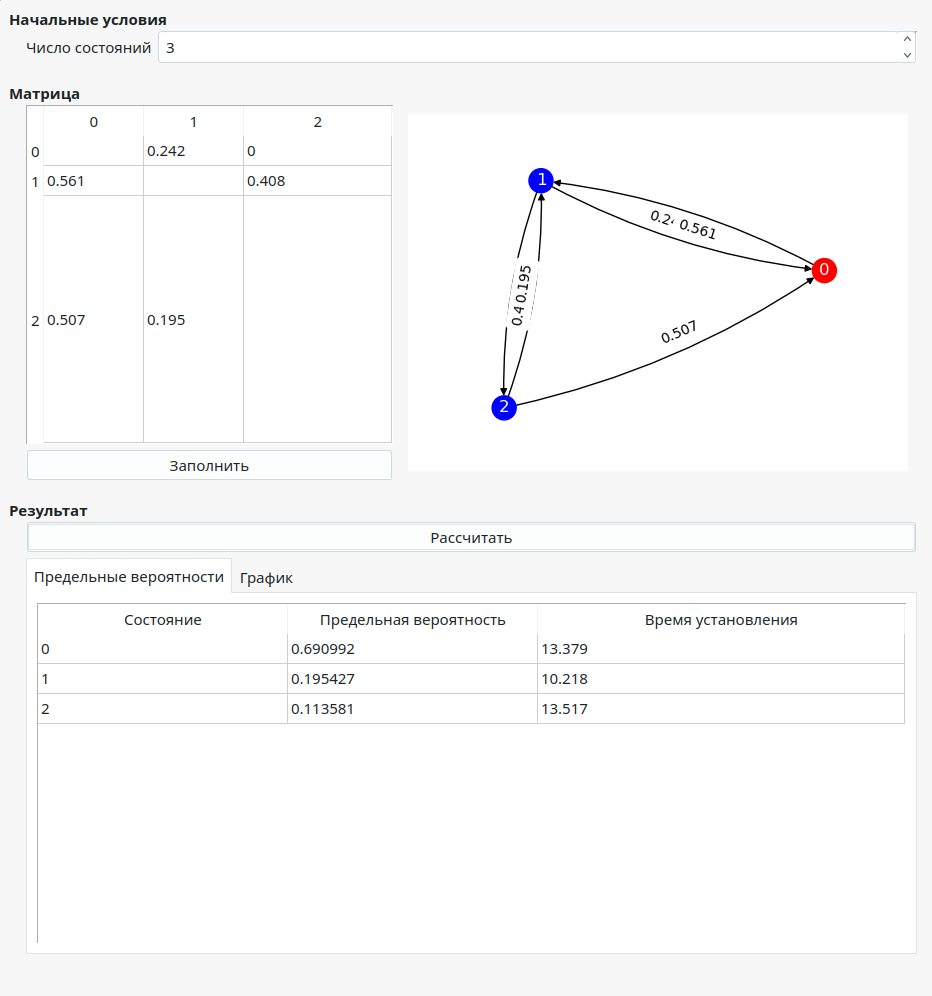
\includegraphics[width=\linewidth]{1.png}
    \end{minipage}
    \hfill
    \begin{minipage}{0.47\textwidth}
        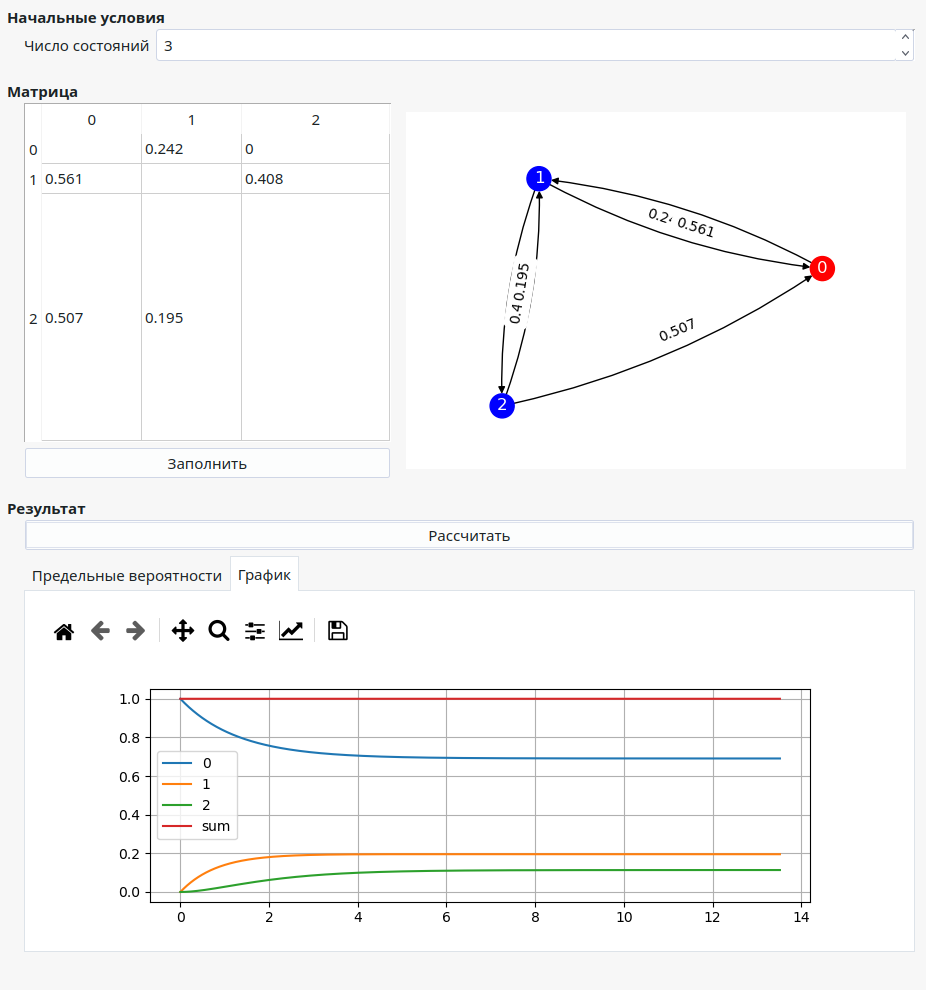
\includegraphics[width=\linewidth]{2.png}
    \end{minipage}
    \caption{Результаты работы программы для системы из трех состояний}
\end{figure}

\clearpage

\section*{Вывод}

В ходе выполнения лабораторной работы была разработана программа, позволяющая
определять среднее относительное время пребывания сложной системы в
предельном стационарном состоянии.

